\ifx \globalmark \undefined %% This is default.
	\documentclass[twoside,openright,11pt,a4paper]{report}

%\compiler avec xelatex
%\usepackage[applemac]{inputenc}
\usepackage[T1]{fontenc}
\usepackage[utf8]{inputenc} %latin1 est possible
%\usepackage[latin1]{inputenc} %latin1 est possible
\usepackage[UKenglish]{babel}
\usepackage{lettrine}

%\usepackage[text={13cm,20cm},centering]{geometry}
\usepackage [squaren, Gray, mediumqspace]{SIunits}
\usepackage [top=2cm, bottom=2cm, left=2cm, right=2cm ]{geometry}

\renewcommand{\familydefault}{cmss}
\addto\captionsenglish{ \renewcommand\chaptername{Solutions of Chapte}}

\usepackage{graphicx}
\usepackage{amsmath}
\usepackage{amsfonts}
\usepackage{amssymb}
\usepackage{amsthm}
\usepackage{bm}
\usepackage{color}

\newcommand{\real}{\mathbb{R}}
\newcommand{\mb}{\mathbf}
\newcommand{\bos}{\boldsymbol}

\def \RR {I \! \! R}

\newcommand{\e}{\begin{equation}}  
\newcommand{\ee}{\end{equation}}
\newcommand{\eqn}{\begin{eqnarray}} 
\newcommand{\eeqn}{\end{eqnarray}} 
\newcommand{\eqnn}{\begin{eqnarray*}} 
\newcommand{\eeqnn}{\end{eqnarray*}} 

\newcommand{\bpm}{\begin{pmatrix}}
\newcommand{\epm}{\end{pmatrix}}

%\newcommand{\{\c c}}{\c c}

\newcommand{\bma}{\left(\begin{array}}
\newcommand{\ema}{\end{array}\right)} 
\newcommand{\hh}{\hspace{2mm}}
\newcommand{\hd}{\hspace{5mm}}
\newcommand{\hu}{\hspace{1cm}}
\newcommand{\vv}{\vspace{2mm}}
\newcommand{\vd}{\vspace{5mm}}
\newcommand{\vm}{\vspace{-2mm}}
\newcommand{\teq}{\triangleq}
%\newcommand{\qedb}{\,$\Box$}
\newcommand{\blanc}{$\left. \right.$}
\newcommand{\frts}[2]%
         {\frac{{\textstyle #1}}{{\textstyle #2}}}

\newcommand{\bindex}[3]%
{
\renewcommand{\arraystretch}{0.5}
\begin{array}[t]{c}
#1\\
{\scriptstyle #2}\\
{\scriptstyle #3}
\end{array}
\renewcommand{\arraystretch}{1}
}

\theoremstyle{definition}
\newtheorem{exemple}{{\bf Exemple}}[chapter]
\newtheorem{theoreme}[exemple]{{\bf Th{é}or{è}me}}
\newtheorem{propriete}[exemple]{{\bf Propri{é}t{é}}}
\newtheorem{definition}[exemple]{{\bf D{é}finition}}
\newtheorem{remarque}[exemple]{{\bf Remarque}}
\newtheorem{remarques}[exemple]{{\bf Remarques}}
\newtheorem{lemme}[exemple]{{\bf Lemme}}
\newtheorem{hypothese}[exemple]{{\bf Hypoth{è}se}}
\newtheorem{exercice}{{\bf Exercice}}[chapter]

\newcommand{\xqedhere}[2]{%
 \rlap{\hbox to#1{\hfil\llap{\ensuremath{#2}}}}}

\newcommand{\xqed}[1]{%
 \leavevmode\unskip\penalty9999 \hbox{}\nobreak\hfill
 \quad\hbox{\ensuremath{#1}}}

\newcommand{\gf}{\fg\,\,}

\newcommand{\cata}[1] %
     {\renewcommand{\arraystretch}{0.5}
     \begin{array}[t]{c} \longrightarrow \\ {#1} \end{array}
     \renewcommand{\arraystretch}{1}}

\usepackage[isu]{caption}
%\usepackage[font=small,format=plain,labelfont=bf,up,textfont=it,up]{caption}
\setlength{\captionmargin}{60pt}

\newcommand{\cqfd}
{%
\mbox{}%
\nolinebreak%
\hfill%
\rule{2mm}{2mm}%
\medbreak%
\par%
}

\pagestyle{headings}

\renewcommand{\sectionmark}[1]{%
\markright{\thesection.\ #1}{}}

\renewcommand{\chaptermark}[1]{%
\markboth{\chaptername\ \thechapter.\ #1}{}}

\makeatletter 
\def\@seccntformat#1{\csname the#1\endcsname.\;} 
\makeatother

\title{ {\Huge {\textbf{Modélisation et analyse  \\ \vspace{4mm} des systèmes dynamiques }}} \\ \vspace{4cm} G. Bastin}

%\title{ {\Huge {\textbf{Modelisation et analyse  \\ \vspace{4mm} des systemes dynamiques }}} \\ \vspace{4cm} G. Bastin}


\date{\today}
	\begin{document} %% Crashes if put after (one of the many mysteries of LaTeX?).
\else 
	\documentclass{standalone}
	\begin{document}
\fi

\graphicspath{ {Chapitre9/images/} }

\setcounter{chapter}{8}
\chapter{Stabilité des équilibres}
\chaptermark{Stabilité des équilibres}\label{stabeq}



\lettrine[lines=1]{\bf C}{}e chapitre traite de la stabilité des équilibres. Plus précisément, on s'intéresse au comportement des trajectoires du système au voisinage des équilibres. Soit un système dynamique décrit par son modèle d'état~:
\e
\dot x = f(x,u). \label{sys}
\ee
On suppose que le système possède un équilibre en $(\bar x, \bar u)$. On se pose les deux questions suivantes~:\\
\begin{itemize}
\item[a:] si l'entrée est maintenue égale à sa valeur d'équilibre $\bar u$
et si l'état initial $x(t_0)$ est dans le voisinage de la valeur d'équilibre
$\bar x$, comment vont se comporter les trajectoires du système ? Sous quelle conditions les trajectoires vont elles converger vers $\bar x$?\\
\item[b:] Si l'entrée $u(t)$ est proche de $\bar u $ (mais pas
nécessairement constante), que
peut-on dire des trajectoires du système ? Sous quelles conditions les trajectoires $x(t)$ resteront-elles proches de $\bar x$?\\
\end{itemize}

\section{Définitions}

\begin{definition} \label{eqstab} {\bf Equilibre stable}

L'équilibre $(\bar x, \bar u)$ est un {\em équilibre stable} du système (\ref{sys}) si 
\eqnn
\forall\epsilon > 0 \;\;\exists \delta>0 \mbox{ t.q.} \| x(t_0)-\bar x\| < \delta
\Rightarrow \| x(t, x(t_0), \bar u) -\bar x \| < \epsilon \;\; \forall t \geq
t_0.
\eeqnn
Si cette condition n'est pas satisfaite, l'équilibre est {\em instable}. \qed
\end{definition}
Cette définition s'interprête de la manière suivante. On souhaite caractériser le fait que la trajectoire $x(t)$ reste proche du point d'équilibre $\bar x$ pour tout $t \geq t_0$ lorsque l'entrée est constante $(u(t) = \bar u \; \forall t \geq t_0$). Pour cela, on mesure la proximité avec la norme $\| \;\;  \|$ et on impose que les solutions $x(t)$ restent à l'intérieur de la région délimitée par $ \| x(t) -\bar x \| < \epsilon$, c'est-à-dire dans un ``tube" de rayon $\epsilon$ autour de la trajectoire $x(t) = \bar x$. Si cet objectif est réalisable pour une condition initiale $x(t_0)$ proche de l'équilibre (c'est-à-dire $ \| x(t_0) -\bar x \| < \delta$), alors on dit que l'équilibre est stable. Sinon, on dit qu'il est instable.

Cette définition est la forme la plus faible de stabilité considérée dans ce chapitre. En particulier, elle n'implique pas que les trajectoires $x(t)$ convergent vers le point d'équilibre.

\begin{definition} \label{eqatt} {\bf Equilibre attracteur}

L'équilibre $(\bar x, \bar u)$ est un {\em équilibre attracteur} de 
(\ref{sys}) si 
\eqnn
\exists \delta>0 \mbox{ t.q.} \| x(t_0)-\bar x \| < \delta
\Rightarrow  \lim_{t \rightarrow \infty} \|x(t, x(t_0), \bar u) -\bar x \|=0. \qed
\eeqnn
\end{definition}
Un équilibre attracteur $\bar x$ est donc un point vers lequel convergent les solutions $x(t)$ si elles démarrent suffisament près de $\bar x$. Il faut noter que stabilité et attractivité sont deux notions différentes et qu'elles ne s'impliquent pas mutuellement. 
\begin{definition} \label{eqast} {\bf Equilibre asymptotiquement stable}

L'équilibre $(\bar x, \bar u)$ est un {\em équilibre asymptotiquement
stable} s'il est stable et attracteur.
\qed
\end{definition}
Un ensemble d'états initiaux $x(t_0)$ à partir desquels les trajectoires convergent vers un équilibre asymptotiquement stable est appelé {\em bassin d'attraction}.
La stabilité asymptotique est la propriété qui est généralement recherchée en pratique. Il faut cependant remarquer que la définition ci-dessus ne nous dit rien sur la vitesse à laquelle la trajectoire $x(t)$ converge vers l'équilibre. C'est pourquoi, on introduit la notion suivante de stabilité exponentielle qui permet de caractériser cette vitesse.
\begin{definition} \label{expstab} {\bf Stabilité exponentielle}

L'équilibre $(\bar x, \bar u)$ est un {\em équilibre exponentiellement
stable} si 
\eqnn
&&\forall\epsilon > 0 \;\;\exists \; a>0, b>0 \mbox{ et } \delta>0 \text{ t.q.} \\ 
&& \| x(t_0)-\bar x \| < \delta 
\Rightarrow \| x(t, x(t_0), \bar u) -\bar x \| \leq a \| x(t_0)-\bar x \|
e^{-bt}\;\; \forall t \geq t_0. \qed
\eeqnn
\end{definition}
Il est évident que la stabilité exponentielle implique la stabilité asymptotique mais l'inverse n'est pas nécessairement vrai.

\section{Première méthode de Lyapunov (méthode indirecte)}

La première méthode de Lyapunov est basée sur l'examen de la linéarisation du système $\dot x = f(x,\bar u)$ autour de l'équilibre $(\bar x, \bar u)$. Plus précisément, on examine les valeurs propres $\lambda_i (A)$ de la matrice Jacobienne évaluée à l'équilibre~:
\eqnn
A = \dfrac {\partial f}{\partial x} (\bar x, \bar u).
\eeqnn
Selon cette méthode, les propriétés de stabilité de $(\bar x, \bar u)$ s'expriment comme suit.

\begin{theoreme}\label{premLyap}{\bf Première méthode de Lyapunov.}

\begin{enumerate}
\item Si toutes les valeurs propres de la matrice Jacobienne ont une partie réelle strictement négative ($\forall i,\;Re(\lambda_i(A))<0$), l'équilibre $(\bar x, \bar u)$ est exponentiellement stable.
\item Si la matrice Jacobienne possède au moins une valeur propre à partie réelle strictement positive ($\exists i, \;Re(\lambda_i(A)) > 0$), l'équilibre $(\bar x, \bar u)$ est instable.
\qed
\end{enumerate}
\end{theoreme}
Le théorème ne permet pas de dire si l'équilibre est stable ou instable quand la matrice Jacobienne comporte au moins une valeur propre nulle et aucune valeur propre à partie réelle strictement positive. Dans ce cas, les trajectoires du système convergent vers un sous-espace
(une variété) dont la dimension est le nombre de valeurs propres nulles de la matrice Jacobienne et la stabilité de l'équilibre peut  être
étudiée dans ce sous-espace par la seconde méthode.

\section{Seconde méthode de Lyapunov (méthode directe)}

Comme nous venons de le voir, la première méthode de Lyapunov est simple à appliquer mais elle ne permet d'analyser la stabilité des équilibres que très partiellement. En outre  elle ne donne aucune indication sur la taille des bassins d'attraction. La seconde méthode est plus difficile à mettre en oeuvre mais, en contrepartie, est d'une portée beaucoup plus générale. Elle est basée sur la définition d'une fonction particulière, notée $V(x)$ et appelée {\em fonction de Lyapunov}, qui est décroissante le long des trajectoires du système à l'intérieur du bassin d'attraction. Avant de donner les différents théorèmes de stabilité, nous commen{\c c}ons par un exemple.

\begin{exemple}\label{exbras}{\bf Un bras de robot à un degré de liberté.}

On considère un bras de robot à un degré de liberté, avec frottement visqueux linéaire et soumis à un couple constant (voir figure ci-dessous). 
Le modèle d'état du système est le suivant (voir chapitre 2 et chapitre 8, section 8.3.1)~:
\begin{equation*} \begin{split}
\dot x_1 &=x_2, \\
\dot x_2 &= J^{-1}(- mgb \sin x_1 - k x_2 + \bar u).
\end{split} \end{equation*}
Dans ces équations, $x_1$ est la position angulaire, $x_2$ la vitesse angulaire, $J$ l'inertie, $m$ la masse, $b$ la distance entre le point d'ancrage et le centre de masse, $k$ le coefficient de frottement et $\bar u$ le couple constant appliqué au bras de robot.

Considérons le cas où $0 < \bar u < mgb$. Le système possède deux équilibres vérifiant les relations suivantes~:
\eqnn
\bar x_1 = \arcsin (\dfrac {\bar u}{mgb}), \hh
\bar x_2 = 0.
\eeqnn
En accord avec l'intuition physique et comme on peut le vérifier en examinant les valeurs propres de la matrice Jacobienne, il y un équilibre asymptotiquement stable en position "basse" et un équilibre instable en position "haute" (voir figure \ref{bras}).
\begin{figure}[h]
\begin{center}
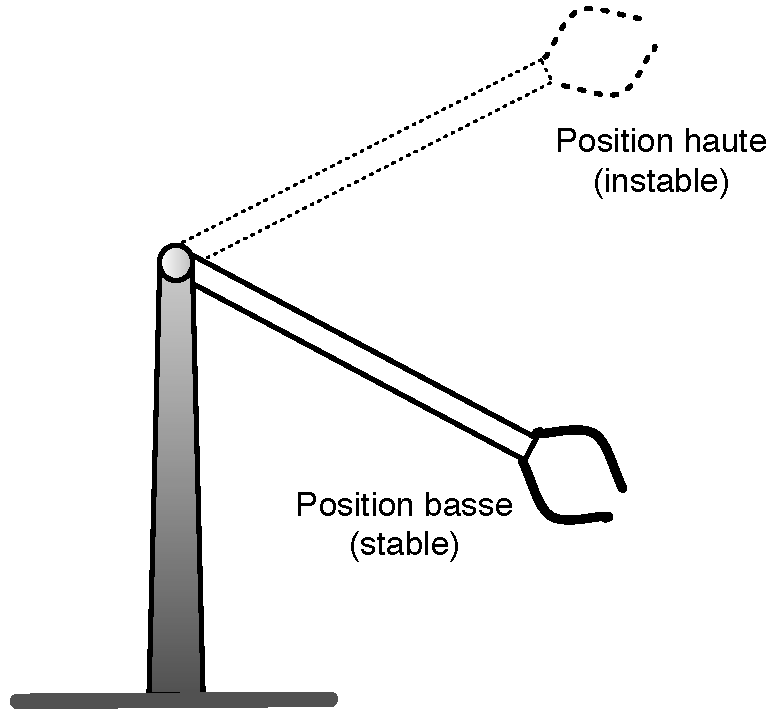
\includegraphics[width=6cm]{bras}
\caption{Bras de robot dans un plan vertical}
\label{bras}
\end{center}
\end{figure}

Considérons la fonction suivante~:  
\eqnn
V(x_1,x_2) = \dfrac {J}{2} x_2^2 +  mgb(1 - \cos x_1) -\bar u x_1. 
\eeqnn
Cette fonction a la dimension d'une énergie. En effet le premier terme ($J x_2^2/2$) est l'énergie cinétique, le second terme ($mgb(1-\cos x_1)$) est l'énergie potentielle et le troisième terme ($\bar u x_1$) est l'énergie dépensée par le couple $\bar u$ pour élever le bras jusqu'à la position angulaire $x_1$ . L'équilibre en position "basse" appartient au domaine
\eqnn
D = \{ (x_1,x_2) : - \pi /2 < x_1 < \pi /2, -a < x_2 < a \}
\eeqnn
(a est un réel positif quelconque).  Dans ce domaine, la fonction $V(x_1,x_2)$ est une fonction qui satisfait les conditions suivantes~:
\begin{itemize}
\item [(i)] $V(x_1,x_2) : D \rightarrow R$ est contin\^ument dérivable.
\item [(ii)] $V(x_1,x_2) > V(\bar x_1, \bar x_2)$ pour tout $(x_1,x_2) \neq (\bar x_1, \bar x_2)$ dans $D$ (c-à-d $V$ est minimum à l'équilibre).
\item [(iii)] $\dot V(x_1,x_2) \leq 0$ en dehors de l'équilibre dans $D$ car
\eqnn
\dot V(x_1,x_2) &=& \dfrac {\partial V}{\partial x_1} \dot x_1+  \dfrac {\partial V}{\partial x_2} \dot x_2 \\
&=& [mgb \sin x_1 - \bar u][x_2] + [J x_2][ J^{-1}(- mgb \sin x_1 - k x_2 + \bar u]\\
&=& - k x_2^2.
\eeqnn
\end{itemize}
Sous ces conditions, comme nous allons le voir avec le théorème suivant, il existe un voisinage borné de l'équilibre dans lequel $V(x_1,x_2)$ décroit le long des trajectoires du système tant que la vitesse $x_2 \neq 0$ et se rapproche du minimum de $V$ qui correspond à l'équilibre. On voit donc que l'équilibre est stable au sens de la définition \ref{eqstab}. On observe cependant que $V(x_1,x_2)$ cesse de décroitre si $x_2=0$ (vitesse nulle). Peut-on avoir une vitesse identiquement nulle  ailleurs qu'à l'équilibre ? En fait non, car une vitesse identiquement nulle implique une accélération identiquement nulle, ce qui implique finalement que le système est à l'équilibre.
\qed
\end{exemple}
Cet exemple illustre l'essentiel de la démarche de la seconde méthode de Lyapunov dont voici le premier théorème.

\begin{theoreme}\label{stabLyap}{\bf Stabilité \og à la Lyapunov \fg.}

L'équilibre $(\bar x, \bar u)$ du système $\dot x = f(x,\bar u)$ est stable si il existe une fonction $V(x): D \rightarrow R$ contin\^ument différentiable ayant les propriétés suivantes~:\\
\begin{itemize}
\item[(i)] $D$ est un ouvert de $R^n$ et $\bar x \in D$;\\
\item[(ii)] $V(x) > V(\bar x)$ $\forall x \neq \bar x$ dans $D$ ($V(x)$ est minimum en $\bar x$);\\
\item[(iii)] $\dot V(x) \leq 0$ $\forall x \neq \bar x$ dans $D$. \qed
\end{itemize}
\end{theoreme}
En d'autres termes, ce théorème veut dire qu'une condition suffisante pour la stabilité de l'équilibre $(\bar x, \bar u)$ est qu'il existe une fonction définie positive $V(x) - V(\bar x)$ dont la dérivée temporelle $\dot V(x)$ est semi-définie négative dans un voisinage de $\bar x$. La dérivée temporelle $\dot V(x)$ se calcule comme suit~:
\eqnn
\dot V(x) = \dfrac {dV}{dt} = \dfrac {\partial V}{\partial x} \dot x = \dfrac {\partial V}{\partial x} f(x, \bar u) = \sum_{i=1}^n \dfrac {\partial V}{\partial x_i} f_i(x, \bar u).
\eeqnn
Les conditions (ii) et (iii) du théorème \ref{stabLyap} impliquent que, pour une constante $c$ suffisamment proche de $V(\bar x)$, l'ensemble~:
\eqnn
\Omega_c = \{ x \in D : V(\bar x) \leq V(x) \leq c \}
\eeqnn
est un compact (c'est-à-dire un ensemble fermé et borné) invariant. Pour le démontrer, 
choisissons une constante positive $r$ telle que la boule fermée
\eqnn
B_r = \{ x \in R^n :  \| x - \bar x \| \leq r \}
\eeqnn
soit contenue dans $D$. Définissons~:
\eqnn
\alpha = \min_{\| x \| = r} V(x).
\eeqnn
Il suffit de choisir n'importe quelle constante $c$ dans l'intervalle ouvert $(0,\alpha)$ pour définir un ensemble $\Omega_c$ qui est inclus dans $B_r$ et donc compact. Supposons maintenant que $x(t_0) \in \Omega_c$. Alors, par la condition (iii), nous avons~:
\eqnn
\dot V(x) \leq 0 \;\;\; \Rightarrow \;\;\; V(\bar x) \leq V(x(t)) \leq V(x(t_0)) \leq c \;\;\; \forall t,
\eeqnn
ce qui montre bien que $\Omega_c$ est invariant.

L'exemple \ref{exbras} est une application de ce théorème qui montre que l'équilibre du bras de robot est stable. En réalité, nous savons intuitivement que cet équilibre est {\em asymptotiquement} stable (c'est-à-dire stable et attracteur). Une manière de démontrer qu'un équilibre est asymptotiquement stable est d'avoir une fonction de Lyapunov dont la dérivée temporelle $ \dot V(x)$ soit strictement  définie négative (et pas seulement semi-définie négative comme dans l'exemple 9.6). Dans ce cas, en effet, la fonction de Lyapunov décroit strictement le long des trajectoires du système, jusqu'à atteindre (asymptotiquement) le minimum qui correspond exactement à l'équilibre.

\begin{theoreme}\label{stabasymp}{\bf Stabilité asymptotique.}

L'équilibre $(\bar x, \bar u)$ du système $\dot x = f(x,\bar u)$ est asymptotiquement stable si il existe une fonction $V(x): D \rightarrow R$ contin\^ument différentiable ayant les propriétés suivantes~:\\
\begin{itemize}
\item[(i)] $D$ est un ouvert de $R^n$ et $\bar x \in D$;\\
\item[(ii)] $V(x) > V(\bar x)$ $\forall x \neq \bar x$ dans $D$ ($V(x)$ est minimum en $\bar x$);\\
\item[(iii)] $\dot V(x) < 0$ $\forall x \neq \bar x$ dans $D$. \qed
\end{itemize}
\end{theoreme}

Comme on l'a vu dans l'exemple du bras de robot, il arrive souvent que l'on trouve une fonction de Lyapunov dont la dérivée est seulement semi-définie négative, ce qui ne permet pas de conclure à la stabilité asymptotique en appliquant le théorème précédent. La difficulté provient notamment de ce que, en analysant la fonction $\dot V(x)$, on n'exploite pas le fait que les différentes variables d'état $x_i$ ne sont pas indépendantes mais sont reliées par les équations de la dynamique du système. LaSalle a étudié cette question en détail et a formulé un principe d'invariance qui permet d'analyser la stabilité asymptotique des équilibres dans le cas d'une fonction $\dot V(x)$ semi-définie négative.
\newpage
\begin{theoreme}\label{lasalle}{\bf Principe d'invariance de LaSalle.}

L'équilibre $(\bar x, \bar u)$ du système $\dot x = f(x,\bar u)$ est asymptotiquement stable si il existe une fonction $V(x): D \rightarrow R$ continument différentiable ayant les propriétés suivantes~:\\
\begin{itemize}
\item[(i)] $D$ est un ouvert de $R^n$ et $\bar x \in D$;\\
\item[(ii)] $V(x) > V(\bar x)$ $\forall x \neq \bar x$ dans $D$ ($V(x)$ est minimum en $\bar x$);\\
\item[(iii)] $\dot V(x) \leq 0$ $\forall x$ dans  $D$;\\
\item[(iv)] l'ensemble $S \subset D$ tel que $\dot V(x) = 0$ ne contient pas de {\em trajectoire} du système autre que $x(t) = \bar x$. \qed
\end{itemize}
\end{theoreme}

\begin{exemple}{\bf  Un bras de robot à un degré de liberté (suite).}

Considérons à nouveau le modèle du bras de robot (voir Exemple \ref{exbras})
\begin{equation} \begin{split} \label{bras}
\dot x_1 &= x_2, \\
\dot x_2 &= J^{-1}(- mgb \sin x_1 - k x_2 + \bar u), 
\end{split} \end{equation}
pour lequel la fonction d'énergie 
\eqnn
V(x_1,x_2) = \dfrac {J}{2} x_2^2 +  mgb(1 - \cos x_1) -\bar u x_1 
\eeqnn
est une fonction de Lyapunov. Le long des trajectoires du système, la dérivée de la fonction de Lyapunov est semi-définie négative~:
\eqnn
\dot V(x_1,x_2)= - k x_2^2 \leq 0.
\eeqnn
L'ensemble $S \subset D$ tel que $\dot V(x) = 0$ est donc le suivant~:
\eqnn
S = \{ (x_1,x_2) \in D : x_2 = 0 \}.
\eeqnn
On observe que toute trajectoire du système contenue dans $S$ est telle que la vitesse $x_2(t)$ est identiquement nulle (ce que nous notons $x_2(t) \equiv 0$). Ceci implique immédiatement que $\dot x_2(t) \equiv 0$. Par l'équation (\ref{bras}), ceci implique que $mgb \sin x_1(t) - \bar u \equiv 0$. Et donc que la seule trajectoire contenue dans $S$ est bien la trajectoire d'équilibre. Donc l'équilibre est asymptotiquement stable. Le raisonnement que nous venons de faire se formalise de la manière suivante~:
\eqnn
\text{trajectoire }(x_1(t),x_2(t)) \in S &\Rightarrow& x_2(t) \equiv 0 \\
&\Rightarrow& \dot x_2(t) \equiv 0 \\
&\Rightarrow& mgb \sin x_1(t) - \bar u \equiv 0 \\
&\Rightarrow& x_1(t) = \bar x_1, x_2(t) = \bar x_2.
\eeqnn
\qed
\end{exemple}

\section{Bassin d'attraction et convergence globale}

Dans la démonstration du théorème \ref{stabLyap} nous avons vu que le domaine $\Omega_c$ est un invariant du système. Si l'équilibre est asymptotiquement stable, cela veut dire que toute trajectoire qui démarre en un point quelconque de $\Omega_c$ converge vers l'équilibre. C'est la raison pour laquelle cet ensemble est appelé "bassin d'attraction". La seconde méthode de Lyapunov nous permet donc de caractériser la taille du bassin d'attraction, information qu'il n'est pas possible d'obtenir par la première méthode. C'est pourquoi il peut être intéressant de chercher une fonction de Lyapunov, même si la stabilité de l'équilibre est facilement démontrée par la linéarisation.

Un cas particulièrement intéressant est quand le point d'équilibre est unique et que le bassin d'attraction contient l'espace d'état tout entier. Dans ce cas, on parle de {\it stabilité asymptotique globale} dont le théorème suivant explicite les conditions d'existence.

\begin{theoreme}\label{stabglob}{\bf Stabilité asymptotique globale.}

L'équilibre $(\bar x, \bar u)$ du système $\dot x = f(x,\bar u)$ est globalement asymptotiquement stable si il est asymptotiquement stable et si en outre~:\\
\begin{itemize}
\item[(i)] $D$ = $\RR^n$;\\
\item[(ii)] $|x| \rightarrow \infty \Rightarrow |V(x)| \rightarrow \infty$. \qed
\end{itemize}
\end{theoreme}

\section{L'énergie comme fonction de Lyapunov}

Le choix d'une fonction de Lyapunov appropriée pour l'analyse de la stabilité des équilibres d'un système dynamique est en général assez difficile.  Comme nous l'a montré l'exemple du robot  à un degré de liberté, l'énergie peut constituer un bon point de départ pour certains systèmes physiques.   Examinons cela sur quelques exemples.\\

\noindent {\bf Systèmes mécaniques}

L'équation générale de la dynamique d'un système mécanique est (cfr Chapitre 2) 
$$
M(q) \ddot q + C(q, \dot q) \dot q + g(q) +k(q) +h(\dot q) =G \bar u
$$
On considère ici le cas particulier où la matrice cinématique $G$ est constante.
Prenons comme fonction $V(q, \dot q)$ la fonction suivante :
$$
V(q,\dot q) = \frac{1}{2} \dot q^T M(q) \dot q + E_{p}(q) - q^TG \bar u
$$
Le premier terme est l'énergie cinétique, le deuxième est l'énergie
potentielle et le troisième correspond au travail des forces et des couples appliqués. La dérivée de cette fonction le long des trajectoires se calcule comme suit~:
\begin{equation*} \begin{split}
\dot V &=  \dfrac{1}{2} \dot q^T[\dot M(q) -2C(q,\dot q)]\dot q -
\dot q^Th(\dot q)\\
&= -\dot q^Th(\dot q),
\end{split} \end{equation*}
(car la matrice $\dot M(q) -2C(q,\dot q)$ est anti-symétrique, voir chapitre 2). Cette grandeur est bien semi-définie négative pour des choix raisonnables de modèles de
frottement visqueux.\\

\noindent {\bf Circuits électriques}

Prenons comme exemple le circuit RLC non linéaire du chapitre 8 (sec. 8.3.1). Les équations d'état sont :
\begin{equation*} \begin{split}
L \dot x_1 &= - r(x_1) - x_2 + \bar u, \\
C \dot x_2 &= x_1.
\end{split} \end{equation*}
Dans ces équations, $x_1$ désigne le courant et $x_2$ la tension. $L$ et $C$ sont l'inductance et la capacité du circuit tandis que $r(x_1)$ est une résistance non-linéaire. Nous supposons que la fonction $r(x_1)$ est monotone croissante et passe par l'origine $r(0)=0$.

Prenons comme fonction de Lyapunov, la fonction suivante qui a la dimension d'une énergie~:
 $$
 V(x_1, x_2) = \dfrac{1}{2}Lx_1^2+\dfrac{1}{2}C(x_2 -\bar u)^2 \geq 0
 $$
 Cette fonction est positive et minimum à l'équilibre $(\bar x_1, \bar x_2) =(0, \bar u)$~: $V(\bar x_1, \bar x_2) = 0$.
D'autre part, on a~:
\begin{equation*} \begin{split}
 \dot V &=  \dfrac{\partial V}{\partial x_1} \dot x_1 +
 \dfrac{\partial V}{\partial x_2} \dot x_2\\
 &= -x_1r(x_1) \leq 0.
\end{split} \end{equation*}
 L'équilibre est donc stable et, en utilisant le principe d'invariance de LaSalle, on peut même conclure à la stabilité asymptotique.\\

\section{Systèmes linéaires}

\noindent Soit le système $\dot x = Ax + B\bar u$ et un équilibre $(\bar x, \bar u)$. On définit comme fonction de Lyapunov $V(x) = (x-\bar x)^T P(x-\bar x)$ où
$P$ est une matrice symétrique définie positive.
\begin{equation*} \begin{split}
\dot V(x) &= \dot x^TP(x-\bar x) +(x-\bar x)^TP\dot x \\
&= (\bar u^TB^T+x^TA^T)P(x-\bar x) +(x-\bar x)^TP(Ax +B\bar u)\\
&= (x-\bar x)^TA^TP(x-\bar x) +(x-\bar x)^TP A(x-\bar x) \\
&= -(x-\bar x)^TQ(x-\bar x),
\end{split} \end{equation*}

\begin{equation} 
\hspace{-5.4cm} \text{avec} -Q = A^TP+PA. \label{SL}
\end{equation}
Cette dernière équation est appelée \og équation matricielle de Lyapunov \fg.  Si
elle admet une solution $Q$ définie positive, alors la fonction $V$ sera
bien une fonction de Lyapunov pour le système.  On peut aussi inverser le raisonnement : on se donne une matrice $Q$ définie positive et on s'appuie sur le théorème suivant pour conclure que la fonction $V$ est bien une fonction de Lyapunov pour le système et que l'équilibre est donc asymptotiquement stable. 

\begin{theoreme}  Soit $A$ une matrice réelle d'ordre $n$.  
Pour toute matrice $Q$ définie positive, (\ref{SL}) possède une solution
unique $P$ définie positive si et seulement si $A$ est une matrice de Hurwitz (toutes ses valeurs propres ont une partie réelle stritement négative).
\qed
\end{theoreme}

\section{Stabilité \og Entrée bornée - Etat borné \fg}
Il est souvent illusoire de pouvoir appliquer une entrée parfaitement constante à un système dynamique réel. En pratique, à cause de diverses sources de perturbation et d'incertitude, l'entrée sera généralement un signal $u(t)$ variant légèrement au voisinage de la valeur d'équilibre désirée. Il est dès lors pertinent de s'intéresser à l'évolution de l'état du système lorsque $u(t)$ est un signal borné proche de $\bar u$. Nous commençons par étudier cette question dans le cas d'un système linéaire
\e \label{systlin}
\dot x = Ax+Bu.
\ee
Pour une condition initiale $x(t_0) = x_0$ et une entrée $u(t)$ données, la trajectoire du système s'écrit explicitement
\eqnn
x(t) = e^{A(t-t_0)}x_0 + \int_{t_0}^t e^{A(t-\tau)} B u(\tau) d \tau.
\eeqnn
Considérons l'équilibre $(\bar x = 0, \bar u = 0)$. Cet équilibre est asymptotiquement stable si et seulement si la matrice $A$ est Hurwitz. Dans ce cas $\| e^{At} \|$ est bornée pour tout $t$ et il existe des constantes positives $k$ et $\lambda$ telles que
\eqnn
\| e^{A(t-t_0)} \| \leq ke^{-\lambda (t-t_0)}.
\eeqnn
On en déduit
\begin{align}
\| x(t) \| &\leq ke^{-\lambda (t-t_0)}\| x_0 \| + \int_{t_0}^t e^{-\lambda(t-\tau)} \| B \| \| u (\tau) \| d \tau \nonumber \\
&\leq ke^{-\lambda (t-t_0)}\| x_0 \| + \dfrac{k \| B \|}{\lambda} \sup_{t_0 \leq \tau \leq t} \| u(\tau) \|. \label{zz}
\end{align}
On voit immédiatement qu'une entrée $u(t)$ bornée, quelle que soit son amplitude, produit bien un état $x(t)$ borné. On observe aussi que l'effet de la condition initiale $x_0$ s'estompe au cours du temps et que la \og borne ultime \fg \, de $x(t)$ est donc simplement proportionnelle à la borne de $u(t)$ :
\eqnn
\limsup_{t \rightarrow +\infty} \| x(t) \| \leq \dfrac{k \| B \|}{\lambda} \| u \|_{{\cal L}_\infty}.
\eeqnn
Voyons maintenant comment ces résultats s'étendent aux systèmes non-linéaires. Nous considérons le système
\eqn \label{systnl}
\dot x = f(x,u) \text{ avec l'équilibre } (\bar x, \bar u)
\eeqn
et nous supposons que la fonction $f(x,u)$ est continûment dérivable dans un voisinage de l'équilibre.

\begin{theoreme}{\bf Stabilité (locale) EBEB}

Si l'équilibre $(\bar x, \bar u)$ du système (\ref{systnl}) est asymptotiquement stable, 
\itemize
\item[(i)] il existe trois constantes positives $c_1$, $c_2$ et $c_3$ telles que, pour tout état initial $x_0$ avec $\|x_0 - \bar x\| < c_1$ et tout signal d'entrée $u(t)$ avec $\| u(t) - \bar u \| < c_2$, la solution $x(t)$ est bornée : $\| x(t) - x_0 \| < c_3$ $\forall t\geq t_0$;
\item[(ii)] il existe une constante positive $c_0$ et une fonction continue $\alpha : [0,a) \rightarrow [0, +\infty)$ passant par l'origine (c-à-d $\alpha(0) = 0$) et croissante\footnote{une telle fonction est dite de classe ${\cal K}$} telle que, pour tout signal d'entrée $u(t)$ avec $\| u(t) - \bar u \| < c_0$ $\forall t\geq t_0$, la \og borne ultime \fg \, de $x(t)$ est une fonction croissante de la borne de $u(t)$ :
\eqnn
\limsup_{t \rightarrow +\infty} \| x(t) \| \leq \alpha( \| u \|_{{\cal L}_\infty}). \qed
\eeqnn
\end{theoreme}

Dans le cas où le système (\ref{systnl}) est défini globalement et possède un équilibre unique, on a aussi la propriété globale suivante.

\begin{theoreme}{\bf Stabilité (globale) EBEB}

Si la fonction $f(x,u)$ est globalement continûment dérivable et globalement Lipschitz en $(x,u)$, si l'équilibre $(\bar x, \bar u)$ est globalement exponentiellement stable, alors 
\itemize
\item[(i)] pour tout état initial $x_0$ et tout signal d'entrée $u(t)$, la solution $x(t)$ est bornée;
\item[(ii)] la \og borne ultime \fg \, de $x(t)$ est une fonction croissante de la borne de $u(t)$.
\qed
\end{theoreme}
Il faut remarquer que ce dernier théorème est assez restrictif. Il existe en effet de nombreux systèmes dynamiques pour lesquels la fonction $f(x,u)$ n'est pas globalement Lipschitz et qui possèdent pourtant une propriété EBEB globale.
Par contre, la condition de stabilité exponentielle de l'équilibre est cruciale. En effet, si l'équilibre est globalement asymptotiquement stable mais pas globalement exponentiellement stable, alors le système (\ref{systnl}) n'est pas nécessairement EBEB stable, même si $f(x,u)$ est globalement Lipschitz.

\section{Exercices}

\begin{exercice}{\bf Un réacteur chimique}

Dans un réacteur continu se déroulent deux réactions chimiques en phase liquide à volume constant faisant intervenir trois espèces chimiques X$_1$, X$_2$, X$_3$. La dynamique du réacteur est décrite par le modèle d'état suivant ($x_i$ désigne la concentration de X$_i$):
\begin{align*}
\dot x_1 &= -x_1^2x_2 - dx_1 + du, \\
\dot x_2 &= x_1^2x_2 - (d+k)x_2, \\
\dot x_3 &= 2kx_2 - dx_3.
\end{align*}
\begin{enumerate}
\item De quelles réactions s'agit-il ? (loi d'action des masses). 
\item Dans l'orthant positif ($x_1 \geq 0$, $x_2 \geq 0$, $x_3 \geq 0$) déterminer le ou les équilibres pour  $\bar u > 0$. Indiquer combien il y a d'équilibres pour chaque valeur de $\bar u$ et expliciter les conditions d'existence. 
\item Analyser la stabilité des équilibres par la première méthode de Lyapunov.
\end{enumerate}
\end{exercice}
\vv

\begin{exercice}{\bf Circuit RLC}

Soit le circuit RLC parallèle illustré ci-dessous :
\begin{figure}[h]
\begin{center}
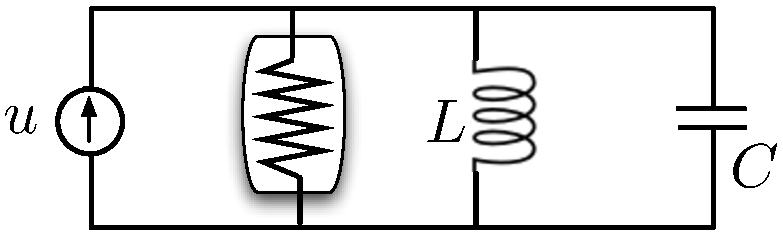
\includegraphics[width=7cm]{RLC1}
\end{center}
\end{figure}

\noindent La caractéristique courant-tension $i=g(v)$ de la résistance non-linéaire est une fonction monotone croissante telle que représentée sur la figure suivante~:
\begin{figure}[h]
\begin{center}
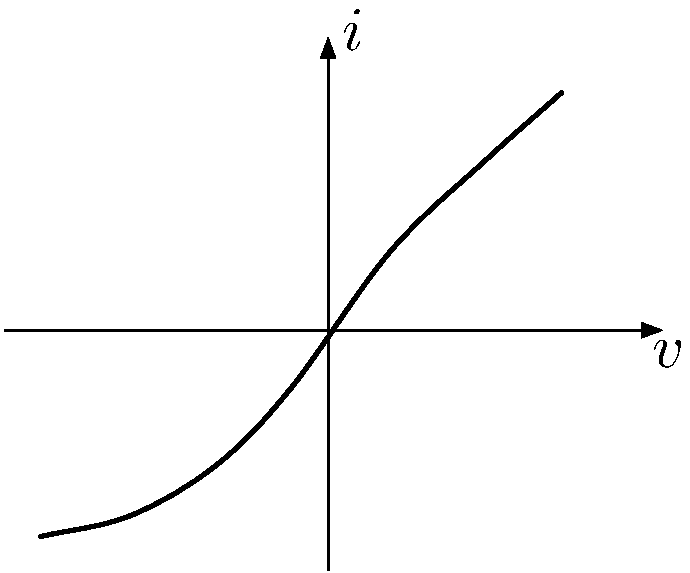
\includegraphics[width=4.8cm]{RLC2}
\end{center}
\end{figure}
\begin{enumerate}
\item Etablir un modèle d'état du système.
\item Calculer les équilibres.
\item En utilisant l'énergie comme fonction de Lyapunov, analyser la stabilité globale des équilibres par la seconde méthode de Lyapunov.
\end{enumerate}
\end{exercice}
\vv

\begin{exercice}{\bf Réacteur chimique}

Soit un réacteur chimique de type CSTR où se produit la réaction suivante
:
$$
X_1 + X_2 \longrightarrow 2X_2.
$$

\begin{enumerate}
\item Etablir un modèle d'état sous les hypothèses de modélisation suivantes
:\\
- cinétique décrite par la loi d'action des masses\\
- réacteur alimenté en $X_1$ uniquement ($x_{1,in} =$ cste)\\
- le débit volumique d'alimentation est l'entrée.
\item Montrer que ce système possède un équilibre dans l'orthant positif.
\item Montrer que $V = x_1-\bar x_1 \ln x_1+x_2-\bar x_2 \ln x_2$ est une
fonction de Lyapunov dans l'orthant positif.
\item Démontrer que l'équilibre est globalement asymptotiquement stable dans
l'orthant positif.
\end{enumerate}
\end{exercice}
\vv

\begin{exercice}{\bf Système mécanique}

On considère un système mécanique à un degré de liberté.  La variable de
position est $x_1$.  Ce système est soumis à une force dérivant d'un potentiel
et à un frottement visqueux linéaire.

L'énergie potentielle est donnée par $$E_p(x_1) = \int^{x_1}_0 \dfrac{\sigma}{K +
|\sigma|} d \sigma.$$\\

\begin{enumerate}
\item Etablir un modèle d'état du système.
\item Calculer les équilibres.
\item Analyser la stabilité des équilibres par la méthode directe de
Lyapunov.
\end{enumerate}
\end{exercice}
\vv

\begin{exercice}{\bf Modélisation d'un neurone}

Le modèle de Naka-Rushton décrivant la dynamique d'un neurone dans la mémoire à court terme est donné par les équations d'état suivantes~:
\eqnn
\dot x_1 = - x_1 + \frac{u x_2}{1+x_2}, \\
\dot x_2 = - x_2 + \frac{u x_1}{1+x_1}.
\eeqnn
\begin{enumerate}
\item Montrer que le système est positif
\item  Analyser l'existence et la stabilité des équilibres dans l'orthant positif (première méthode de Lyapunov).
\item Pour $u$ constant, $0 < \bar u < 1$, montrer que toutes les trajectoires dans l'orthant positif convergent vers l'origine à l'aide de la fonction de Lyapunov $V = (1/2) (x_1^2 + x_2^2)$.
\end{enumerate}
\end{exercice}
\vv

\begin{exercice} Soit le système dynamique :
\eqnn
\dot x_1 &=& -x_1+x_2,\\
\dot x_2 &=& -x^3_1(1+u^2).
\eeqnn
Avec une fonction de Lyapunov de la forme
$$V = ax^\alpha_1 + bx^\beta_2$$
où $a, b, \alpha, \beta$ sont des constantes positives à
déterminer, montrer que, pour toute entrée constante $u(t) = \bar u$, ce système possède un équilibre unique et
globalement asymptotiquement stable.
\end{exercice}
\vv

\begin{exercice}
Soit le systèmes dynamique :
\begin{align*}
\dot x_1 &= - \phi(x_1) + \phi(x_2), \\
\dot x_2 &= \phi(x_1) - 2 \phi(x_2) + u.
\end{align*}
La fonction $\phi(x) : \RR \longrightarrow \RR$ possède les propriétés suivantes :\\
\begin{itemize}
\item[a)] $\phi(x)$ est une bijection,\\
\item[b)] $\phi(x)$ est $C^\infty$,\\
\item[c)] $\phi(x)$ est strictement monotone croissante ($d\phi$/$dx$ $> 0$, $\forall x \in \RR$),\\
\item[d)] $\phi(x)$ passe par l'origine ($\phi(0) = 0$).
\end{itemize}
\vspace{8mm}
\noindent 1. Démontrer qu'il s'agit d'un système à compartiments. \\

\noindent 2. Pour une entrée constante strictement positive ($\bar u > 0$), expliciter les conditions sous lesquelles le système possède un équilibre unique dans l'orthant positif.\\

\noindent 3. Démontrer que cet équilibre, s'il existe, est globalement asymptotiquement stable à l'aide de la fonction de Lyapunov
\begin{equation*}
V(x_1,x_2) = \int_{\bar x_1}^{x_1} (\phi(s) - \bar u) ds + \int_{\bar x_2}^{x_2} (\phi(s) - \bar u) ds.
\end{equation*}

\end{exercice}

\end{document}
